\documentclass[cjk,dvipdfmx,10pt,compress,%
hyperref={bookmarks=true,bookmarksnumbered=true,bookmarksopen=false,%
colorlinks=false,%
pdftitle={第 105 回 関西 Debian 勉強会},%
pdfauthor={倉敷・のがた・佐々木・かわだ},%
%pdfinstitute={関西 Debian 勉強会},%
pdfsubject={資料},%
}]{beamer}

\title{第 105 回 関西 Debian 勉強会}
\subtitle{$\sim$発表資料$\sim$}
\author[かわだ てつたろう]{{\large\bf 倉敷・のがた・佐々木・かわだ}}
\institute[Debian JP]{{\normalsize\tt 関西 Debian 勉強会}}
\date{{\small 2015 年 12 月 27 日}}

%\usepackage{amsmath}
%\usepackage{amssymb}
\usepackage{graphicx}
\usepackage{moreverb}
\usepackage[varg]{txfonts}
\AtBeginDvi{\special{pdf:tounicode EUC-UCS2}}
\usetheme{Kyoto}
\def\museincludegraphics{%
  \begingroup
  \catcode`\|=0
  \catcode`\\=12
  \catcode`\#=12
  \includegraphics[width=0.9\textwidth]}
%\renewcommand{\familydefault}{\sfdefault}
%\renewcommand{\kanjifamilydefault}{\sfdefault}
\begin{document}
\settitleslide
\begin{frame}
\titlepage
\end{frame}
\setdefaultslide

\begin{frame}[fragile]
  \frametitle{Disclaimer}
  \begin{itemize}
  \item 疑問、質問、ツッコミ、茶々、\alert{大歓迎}
  \item その場でインタラクティブにどうぞ
  \item ハッシュタグ \#kansaidebian
  \end{itemize}
\end{frame}

\begin{frame}[fragile]
\frametitle{Agenda}

\tableofcontents

\end{frame}

\section{最近の Debian 関係のイベント}

\takahashi[40]{最近の Debian\\関係のイベント}

\begin{frame}[fragile]
  \frametitle{第104回関西Debian勉強会}
  \begin{itemize}
  \item 日時: 11月22日(日)
  \item 場所: 福島区民センター
  \end{itemize}
  \begin{block}{内容}
    \begin{itemize}
    \item ライトニングトーク
      \begin{itemize}
      \item Skylakeを使ってみた
      \end{itemize}
    \end{itemize}
  \end{block}
\end{frame}

\begin{frame}[fragile]
  \frametitle{第134回東京エリアDebian勉強会}
  \begin{itemize}
  \item 日時: 12月19日(土)
  \item 場所: イベント&コミュニティスペース dots.
  \end{itemize}
  \begin{block}{内容}
    \begin{itemize}
    \item 「Debianおすすめのパッケージを参加者に聞いてみた」
    \item 「Debianモバイルwifiルータ化」
    \end{itemize}
  \end{block}
\end{frame}

\begin{frame}[fragile]
  \frametitle{Debian Project}
  \begin{itemize}
  \item Perl 5.22 transition underway
  \item glibc 2.21
  \item OpenSSH 7.0
  \item Bits from the Debian Continuous Integration project
  \item AppStream / DEP-11 support now available in the Debian archive
  \item Rename security suite to *-security
  \item Packages with /outdated/ packaging style
  \item Upcoming stable point release (8.3)
  \end{itemize}
\end{frame}

\takahashi[50]{そんな\\こんなで}
\takahashi[120]{次}

\takahashi[50]{事前課題}

\begin{frame}[fragile]
  \frametitle{事前課題}
  \begin{block}{今回の事前課題}
    \begin{description}
    \item[事前課題1]
      2016年関西Debian勉強会ネタ
    \end{description}
  \end{block}
\end{frame}

\takahashi[50]{事前課題\\発表}

\begin{frame}
  \frametitle{ Yuki Okuno }
  \begin{enumerate}
  \item Debian LTS
  \end{enumerate}
\end{frame}

\begin{frame}
  \frametitle{ 矢吹 幸治 }
  \begin{enumerate}
  \item がちゃぴん先生デバッグ三種類
  \end{enumerate}
\end{frame}

\begin{frame}
  \frametitle{ 木下 聖士 }
  \begin{enumerate}
  \item 黒鼓
  \end{enumerate}
\end{frame}

\begin{frame}
  \frametitle{ 榎真治 }
\end{frame}

\begin{frame}
  \frametitle{ 佐々木洋平 }
  \begin{enumerate}
  \item DDになる
  \item systemd-networkd
  \end{enumerate}
\end{frame}

\begin{frame}
  \frametitle{ Yosuke OTSUKI }
  \begin{enumerate}
  \item OpenFOAM
  \end{enumerate}
\end{frame}

\begin{frame}
  \frametitle{ t3rkwd }
  \begin{enumerate}
  \item 運営助けて
  \item gbp
  \item 定番ネタ(パッケージング、ライセンスなど)
  \end{enumerate}
\end{frame}

\begin{frame}
  \frametitle{ nogajun }
  \begin{enumerate}
  \item Debian Live
  \item docker
  \end{enumerate}
\end{frame}

\begin{frame}
  \frametitle{ Yamada Yohei (山田 洋平) }
  \begin{enumerate}
  \item Window Manager
  \end{enumerate}
\end{frame}

\begin{frame}
  \frametitle{ 川江 浩 }
  \begin{enumerate}
  \item GNU Hurd (1月)
  \end{enumerate}
\end{frame}

\takahashi[50]{そんな\\こんなで}
\takahashi[120]{次}

\section{LibreOfficeの最近の動向とDebianでのLibreOfficeパッケージについて}
\takahashi[30]{LibreOfficeの最近の動向とDebianでのLibreOfficeパッケージについて\\by\\榎 真治}

\section{2015年の振り返りと2016年の企画}
\takahashi[30]{2015年の振り返りと2016年の企画\\by\\Debian JP}

\takahashi[50]{2015年を\\振り返って}
\begin{frame}
  \frametitle{今年のお題一覧}
  {\footnotesize
    \vspace{1em}
    \begin{table}
      \centering
    \begin{tabular}{|l|c|l|p{26em}|}
      \hline
      開催年月  & 参加 & 内容 \\
      \hline
        2015年1月 &5      & Debian Bug Squashing Party \\
      \hline
        2015年1月 &5      & {\color<2->[rgb]{1,0,0}{Debian の Bug の眺め方}}, Bug Squash Party \\
      \hline
        2015年2月 &3      & もくもくの会 \\
      \hline
        2015年3月 &7      & {\color<2->[rgb]{1,0,0}{某所 VPS を先走って Jessie に上げてみた}} \\
      \hline
        2015年4月 &14     & Debian 8 "Jessie" Release Party \\
      \hline
        2015年5月 &5      & Jessie落穂拾い \\
      \hline
        2015年6月 &7      & Wheezy→Jessieで踏み抜いた地雷のご紹介 \\
      \hline
        2015年7月 &13     & \color<3->[rgb]{0,0,1}{OSC 2015 Kansai @ Kyoto} \\
      \hline
        2015年8月 &8      & {\color<2->[rgb]{1,0,0}{wiki:Subkeys}} \\
      \hline
        2015年9月 &7      & {\color<2->[rgb]{1,0,0}{ドイツ、ハイデルベルクで開催されたDebconf15へいってきました}} \\
      \hline
        2015年11月&32     & \color<3->[rgb]{0,0,1}{KOF 2015} \\
      \hline
        2015年11月&4      & ライトニングトーク, もくもくの会 \\
      \hline
        2015年12月&9      & 2015年の振り返りと2016年の企画, 忘年会 \\
      \hline
    \end{tabular}
    \end{table}
  }
\end{frame}

\begin{frame}
  \frametitle{2015年の参加状況}
  \centering
  関西の参加人数推移(参加人数と6ヶ月移動平均、アンケート回答人数)
  \begin{figure}[h]
    \begin{center}
      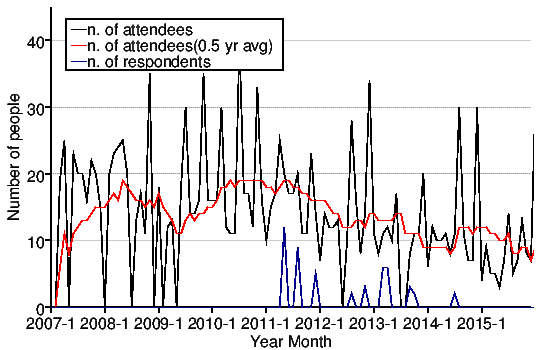
\includegraphics[width=.6\hsize]{image201512/memberanalysis/kansai.png}
    \end{center}
  \end{figure}
\end{frame}

\begin{frame}
  \frametitle{今年のイベント/お題}
  \begin{itemize}
  \item もくもくの会
  \item \color[rgb]{1,0,0}{セッション}
    \begin{itemize}
    \item Debian の Bug の眺め方, 某所 VPS を先走って Jessie に上げてみた,
      wiki:Subkeys, ドイツ、ハイデルベルクで開催されたDebconf15へいってきました
    \end{itemize}
  \item \color[rgb]{0,0,1}{イベント}
    \begin{itemize}
    \item OSC 2015 Kansai@Kyoto, KOF 2015
    \end{itemize}
  \end{itemize}
\end{frame}

\begin{frame}
  \frametitle{定例ネタ(パッケージ作成, バグ報告など)}
  \begin{exampleblock}{背景・目的}
    {\small{
        2007年度から関西でも Debian 勉強会を始動しています。
        \alert{短期的な目標は、Debian Developer(Debian開発者,以下DD) を増やすことです。}
        東京ではDebian勉強会が開催されてきましたが、一方の関西は、東京にくらべて DD の数が少ないです。 関西 Debian 勉強会は、DD と出会って GPG Key Sign をするチャンスを提供します。 また、勉強会を行うことを通して、Debian に関する知識を共有します。}}
    \vskip.5em
    \hspace*\fill{\small--- http://wiki.debian.org/KansaiDebianMeeting}
  \end{exampleblock}
  \begin{itemize}
  \item Bug Squashing Party, Release Party, Upgrade
    \begin{itemize}
    \item リリースに関わる内容
    \end{itemize}
  \item DD 以外での貢献
  \end{itemize}
\end{frame}

\begin{frame}
  \frametitle{運営}
  \begin{itemize}
  \item 運営フロー
  \item ネタの見直し
  \item リソース不足
  \end{itemize}
\end{frame}

\begin{frame}
  \frametitle{イベント}
  \begin{itemize}
  \item 定例は以下の通り
    \begin{description}
    \item[OSC Kansai@Kyoto] \mbox{~}\\
      来年も8月
    \item[KOF 2016] \mbox{~}\\
      来年も11月
    \end{description}
  \end{itemize}
\end{frame}

\takahashi[50]{2016年の企画}
\begin{frame}
  \frametitle{2016年の企画}
  \begin{itemize}
  \item GNU Hurd (1月, 川江)
  \item systemd-networkd (2月, 佐々木)
  \item Open FOAM (4月, OTSUKI)
  \item パッケージング, ライセンス などの定例ネタ
  \item パッケージング道場 (サイボウズさんに交渉してみる?)
  \item もくもくの会
    \begin{itemize}
    \item 成果発表をやる
    \item テーマを決める
    \end{itemize}
  \item Window Manager
  \item Bug Squash
  \item がちゃぴん先生デバッグ三種類
  \end{itemize}
\end{frame}

\begin{frame}
  \frametitle{2016年の開催日}
  \begin{itemize}
  \item 1月24日({\color{red}日}) 福島区民センター 304号
  \item 2月28日({\color{red}日}) 福島区民センター 304号
  \item 3月27日({\color{red}日}) 福島区民センター 304号
  \item 4月23日({\color{blue}土}) 港区区民センター 梅
  \item 4月24日({\color{red}日}) 福島区民センター 304号
  \item 5月21日({\color{blue}土}) 福島区民センター 304号
  \item 5月22日({\color{red}日}) 福島区民センター 304号
  \end{itemize}
\end{frame}

\takahashi[50]{そんな\\こんなで}
\takahashi[50]{来年も頑張りましょう}

\takahashi[120]{次}

\section{今後の予定}
\begin{frame}[fragile]
\frametitle{今後の予定}

\begin{block}{第106回関西Debian勉強会}
  \begin{itemize}
  \item 日時: 1月24日(日)
  \item 場所: 福島区民センター
  \end{itemize}
\end{block}

\begin{block}{第135回東京エリアDebian勉強会}
  \begin{itemize}
  \item 日時: 1月23日(土)
  \item 場所: イベント&コミュニティスペース dots.
  \end{itemize}
\end{block}

\end{frame}

\takahashi[50]{  }

\end{document}
%%% Local Variables:
%%% mode: japanese-latex
%%% TeX-master: t
%%% End:
